\documentclass[14pt]{extarticle} % zmienić na 14 przed wyslaniem tj

\usepackage[T1]{fontenc}
\usepackage[utf8]{inputenc}

\usepackage[hidelinks]{hyperref}

\usepackage{microtype}

\usepackage{amssymb}
\usepackage{amsmath}
\usepackage{mathtools}
\usepackage{dsfont}

\usepackage{enumitem}

\usepackage{tikz}
\usetikzlibrary{cd, patterns, patterns.meta, decorations.pathmorphing}

\usepackage{geometry}
\geometry{a4paper, total={170mm, 252mm}, top=22mm}

\usepackage[skip=7pt]{parskip}

\usepackage{amsthm}
\usepackage{thmtools}

\declaretheoremstyle[
    headfont=\bfseries\color{green!80!black},
    bodyfont=\normalfont,
    notebraces={: }{},
    notefont=\color{green},
    headformat=\NAME$\;$\NUMBER\NOTE,
    postheadspace=\newline,
    mdframed={
        linewidth=2pt,
        rightline=false, topline=false, bottomline=false,
        linecolor=green, backgroundcolor=yellow!4,
        skipabove=3mm, skipbelow=3mm
    }
]{defbox}

\declaretheoremstyle[
    headfont=\bfseries\color{orange!80!black},
    bodyfont=\normalfont,
    notebraces={: }{},
    notefont=\color{orange},
    headformat=\NAME$\;$\NUMBER\NOTE,
    postheadspace=\newline,
    mdframed={
        linewidth=2pt,
        rightline=false, topline=false, bottomline=false,
        linecolor=orange, backgroundcolor=yellow!4,
        skipabove=3mm, skipbelow=3mm
    }
]{theorembox}

\declaretheoremstyle[
    headfont=\bfseries\color{blue!80!black},
    bodyfont=\normalfont,
    notebraces={: }{},
    notefont=\color{purple},
    headformat=\NAME$\;$\NUMBER\NOTE,
    postheadspace=\newline,
    mdframed={
        linewidth=2pt,
        rightline=false, topline=false, bottomline=false,
        linecolor=purple, backgroundcolor=yellow!4,
        skipabove=3mm, skipbelow=3mm
    }
]{lemmabox}

\declaretheoremstyle[
    headfont=\bfseries\color{orange!80!black},
    bodyfont=\normalfont,
    notebraces={: }{},
    notefont=\color{orange},
    headformat=\NAME$\;$\NUMBER\NOTE,
    postheadspace=\newline,
    mdframed={
        linewidth=2pt,
        rightline=false, topline=false, bottomline=false,
        linecolor=red!50!orange, backgroundcolor=yellow!4,
        skipabove=3mm, skipbelow=3mm
    }
]{conclusionbox}

\newtheoremstyle{straightstyle}
  {6pt} % Space above
  {6pt} % Space below
  {} % Body font
  {} % Indent amount
  {\bfseries} % Theorem head font
  {.} % Punctuation after theorem head
  {.5em} % Space after theorem head
  {} % Theorem head spec (can be left empty, meaning `normal')

\newtheoremstyle{italicsstyle}
  {6pt} % Space above
  {6pt} % Space below
  {\slshape} % Body font
  {} % Indent amount
  {\bfseries} % Theorem head font
  {.} % Punctuation after theorem head
  {.5em} % Space after theorem head
  {} % Theorem head spec (can be left empty, meaning `normal')

\declaretheorem[ %
  name=Definition, %
  numberwithin=section, %
  style=defbox
]{definition}

\declaretheorem[ %
  name=Theorem, %
  numberwithin=section, %
  style=theorembox
]{theorem}

\declaretheorem[ %
  name=Proposition, %
  numberlike=theorem, %
  style=theorembox
]{proposition}

\declaretheorem[ %
  name=Corollary, %
  numberlike=theorem, %
  style=straightstyle
]{corollary}

\declaretheorem[ %
  name=Lemma, %
  numberlike=theorem, %
  style=lemmabox
]{lemma}

\declaretheorem[ %
  name=Remark, %
  numberlike=definition, %
  style=italicsstyle
]{remark}



\declaretheorem[ %
  name=Conclusion, %
  numberlike=theorem, %
  style=conclusionbox
]{conclusion}

\declaretheorem[ %
  name=Example, %
  numberwithin=section, %
  style=straightstyle
]{example}



% \renewenvironment{proof}{{\bfseries Proof}$ $\newline}{
%   \begin{flushright} $ \spadesuit $ \end{flushright}$ $\newline
% }

\usepackage{cleveref}

%\crefname{definition}{definicja}{definicje}
%\Crefname{definition}{Definicja}{Definicje}
%
%\crefname{theorem}{twierdzenie}{twierdzenia}
%\Crefname{theorem}{Twierdzenie}{Twierdzenia}
%
%\crefname{lemma}{lemat}{lematy}
%\Crefname{lemma}{Lemat}{Lematy}
%
%\crefname{remark}{uwaga}{uwagi}
%\Crefname{remark}{Uwaga}{Uwagi}


\DeclareMathOperator{\Z}{\mathbb{Z}}
\DeclareMathOperator{\R}{\mathbb{R}}
\DeclareMathOperator{\C}{\mathbb{C}}
\DeclareMathOperator{\N}{\mathbb{N}}
\DeclareMathOperator{\Q}{\mathbb{Q}}

\DeclareMathOperator{\im}{im}
\DeclareMathOperator{\coker}{coker}

\newcommand{\set}[1]{\mathcal{#1}}


\DeclareMathOperator{\ord}{ord}
\DeclareMathOperator{\Ann}{Ann}
\DeclareMathOperator{\Hom}{Hom}

\DeclareMathOperator{\End}{End}

\let\landtemp\land
\renewcommand{\land}{\;\landtemp\;}





\usepackage{tikz}
\usetikzlibrary{spath3, hobby, knots, braids}

\pgfdeclarelayer{bg}    % declare background layer
\pgfsetlayers{bg,main}

\title{A voyage into the algebras}
\author{
  Weronika Jakimowicz\\
  330006
  \and 
  Julia Walczuk\\
  332742
}
\date{2023-2024}

% \definecolor{red}{HTML}{000000}
% \definecolor{blue}{HTML}{000000}
% \definecolor{orange}{HTML}{000000}
% \definecolor{green}{HTML}{000000}

\begin{document}
\maketitle
\bigskip

\begin{center}
  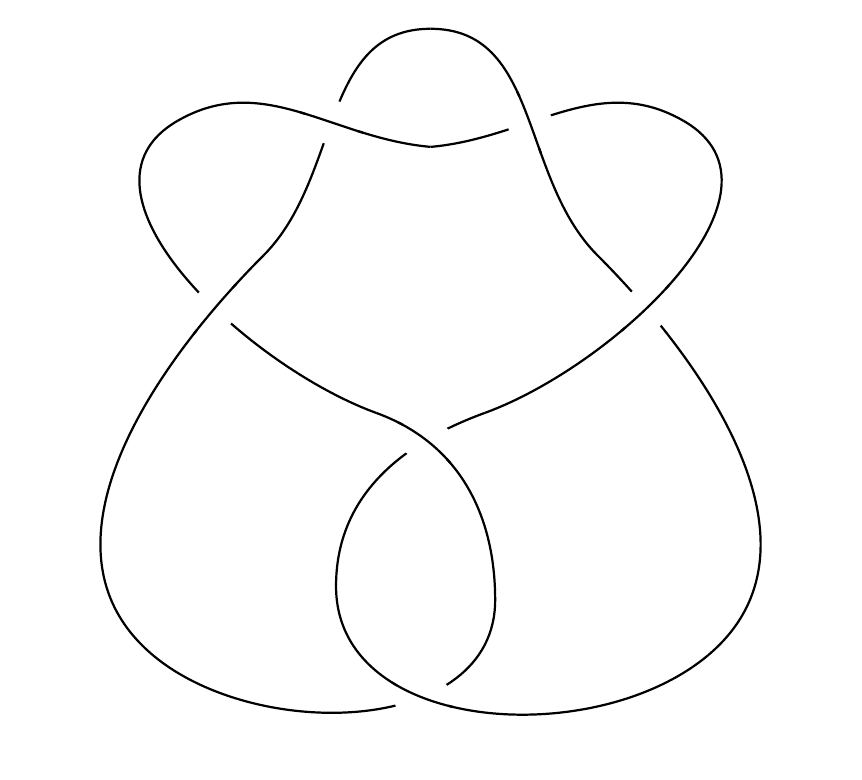
\begin{tikzpicture}[bgnd/.style={circle, fill=white, draw=white}]
    %\node[opacity=0.2] at (0,0) {\includegraphics[width=0.7\textwidth]{./rozdzialy/6_1-3d.png}};

    \coordinate (a0) at (0,0);
    \coordinate (a1) at (90:5);
    \coordinate (a2) at (45:3);
    \coordinate (a3) at (-40:4.6);
    \coordinate (a4) at (-120:2.4);
    \coordinate (a5) at (10:0.7);
    \coordinate (a6) at (50:5);
    \coordinate (a7) at (90:3.5);
    \coordinate (a8) at (180-50:5);
    \coordinate (a9) at (170:0.7);
    \coordinate (a10) at (-70:2.4);
    \coordinate (a11) at (220:4.6);
    \coordinate (a12) at (180-45:3);

    %\foreach \i in {0,...,12} \fill (a\i) circle (2pt);

    \begin{knot}[
      clip width=20, 
      flip crossing=1,
      flip crossing=3,
      flip crossing=6
      ]
      \strand[thick] (a1) to[out=0, in=90+45] (a2) to[out=-45, in=40] (a3);
      \strand[thick] (a3) to[out=220, in=-90] (a4) to[out=90, in=200] (a5);
      \strand[thick] (a5) to[out=20, in=-30] (a6);
      \strand[thick] (a6) to[out=150, in=5] (a7);
      \strand[thick] (a7) to[out=175, in=30] (a8);
      \strand[thick] (a8) to[out=210, in=160] (a9);
      \strand[thick] (a9) to[out=-20, in=90] (a10);
      \strand[thick] (a10) to[out=-90, in=-40] (a11);
      \strand[thick] (a11) to[out=140, in=180+45] (a12);
      \strand[thick] (a12) to[out=45, in=180] (a1);
    \end{knot}
  \end{tikzpicture}
\end{center}

\newpage

\section{Knot coloring}

Let $R$ be any commutative ring with identity, let $M$ be a module with one generator and $\phi:M^3\to M$ be a homomorphism such that for every $m\in M$
%$M$ be any \textbf{\color{red}finitely generated} $R$-module and $\phi:M^3\to M$ be a homomorphism such that for every $m\in M$ 
\begin{equation}\label{phi allows for trivial colorings}
  \phi(m,m,m)=0.
\end{equation}
Notice that if $\phi(u,i,o)=au+bi+co$, then aforementioned equality demands that $(a+b+c)\in \ann(M)$.

Take $K$ to be any knot with diagram $D$ with $s$ arches and $x$ crossings.

\begin{lemma}
  For diagrams of knots other than $0_1$, the number of segments $s$ is equal to the number of crossings $x$.
\end{lemma}

\begin{proof}
  Every crossing has $2$ arcs that go below it and every arc has two bottom ends that are created when this segment disappears below another segment. Thus 
  $$2\cdot \#\text{arches} = \#\text{bottom ends} = 2\cdot \#\text{crossings}.$$
\end{proof}

\begin{definition}\label{coloring definition primitive}
  We say that $C\subseteq M^s$ is a \emph{coloring module} of the diagram $D$ with elements from $M$ if it 
  \begin{enumerate}
    \item {\color{orange}has $s$ generators, each corresponding to one arc of the diagram}, 
    \item and for every $u, i, o\in C$ that correspond to arcs meeting in one crossing, $\phi(u,i,o)=0$.
  \end{enumerate}
  \begin{center}
    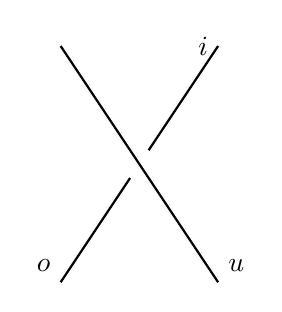
\begin{tikzpicture}
      \draw[thick] (0,0) node[above left] {$o$} --(2, 3) node [left] {$i$};
      \fill[white] (1, 1.5) circle (6pt);
      \draw[thick] (0, 3)--(2, 0) node[above right] {$u$};
    \end{tikzpicture}
  \end{center}
\end{definition}

Notice that condition stated in \cref{phi allows for trivial colorings} makes it possible to color every diagram trivially, that is by assigning the same element of $M$ to every arc of $D$.

Approach to coloring taken in \cref{coloring definition primitive} gives a lot of information about coloring with elements of one specific module $M$ and if one was to change the module to some $M'\neq M$, almost all information gathered for previous coloring would be now ineffectual. Consider the following example.
%it is rather difficult to extrapolate it for other modules. Consider the following example.
%it is rather difficult to use it for other modules. Consider the following example.

\begin{example}
  Take $R=\Z$ with $\phi(x, y, z)=2x-y-z$ and consider the trefoil knot $3_1$. If we take $M=\Z$ then $K$ admits only the trivial coloring module: 
  $$C_M=\{(x, x, x)\;:\;x\in\Z\}.$$ 
  However, if we take $M'=\Z_3$ then there exists a non-trivial coloring like the one presented in \cref{trefoil knot diagram 1}.
  \begin{figure}[h]\centering
    \begin{tikzpicture}[bgnd/.style={circle, fill=white, draw=white}]
       \begin{knot}[
         consider self intersections,
         flip crossing=2,
         clip width=20,
         ]
         \strand[thick]
         (90:3) to[out=180,in=-120,looseness=2]
         (-30:3) to[out=60,in=120,looseness=2]
         (210:3) to[out=-60,in=0,looseness=2] (90:3);
       \end{knot}

       \node[bgnd] at (90:3) {$0$};
       \node[bgnd] at (-30:3) {$1$};
       \node[bgnd] at (210:3) {$2$};
  \end{tikzpicture}
 \caption{The trefoil knot $3_1$ does not allow for nontrivial coloring over $M=\Z$ but it is possible to color it with $M=\Z_3$.\label{trefoil knot diagram 1}}
\end{figure}
\end{example}

Another approach to defining coloring module of a knot diagram $D$ would be by starting with identifying arches with generators $(0,..., 1, ..., 0)$ of $M^s$. Then, we might define a homomorphism
$$f:M^s\to M^x$$
such that arches building one crossing follow rules set by $\phi$.

% We might want to start defining coloring by defining a homomorphism
% $$f:M^s\to M^x$$
% which identifies coordinates with arcs in $D$ and follows $\phi$ on triples of coordinates that build one crossing. 

\begin{definition}\label{coloring definition as kernel}
  Module $\ker f$ is a coloring module of diagram $D$ with elements of $M$.
\end{definition}

Henceforth, we will call $f$ described above a \textbf{coloring homomorphism} for chosen $R$, $M$ and $\phi$.

\begin{corollary}\label{rownowaznosc definicji}
  \Cref{coloring definition primitive} and \cref{coloring definition as kernel} are equivalent for one dimensional modules.
\end{corollary}

\begin{proof}
  {\large\color{red}TO DO}
\end{proof}

Despite the fact that it is the kernel of $f$ that contains colorings, examining the coloring homomorphism itself gives more information about diagram $D$. We might consider $f$ as a $s\times s$ matrix and if $R$ is a PID module, then we can represent this matrix in Smith's normal form. 
%This representation contains information about the kernel over the specific module $M$ and ring $R$ but also shows how to change $M$ and even $R$ to obtain a different coloring.

\begin{proposition}
  Let $A$ be the Smith's normal form of $f$. Columns of $A$ comprised only of zeros and zero divisors contribute to the coloring module. %Moreover, non-unit elements that appear on the diagonal hint at what other colorings are admissible.
\end{proposition}

\begin{proof}
  An immediate result of \cref{rownowaznosc definicji}. The second part 
%  {\large\color{red}TUTAJ WOGÓLE POTRZEBA COKOLWIEK DOWODZIĆ?}
\end{proof}

%Furthermore, if $R$ is a Noetherian ring, then every finitely generated module is a quotient of a free module with the same number of generators. Thus, taking $M$ to be any finitely generated module over $R$ gives us information about coloring with any other module with equal number of generators.

{\color{blue}
If $R$ is a Noetherian ring, then every finitely generated module is a quotient of a free module with the same number of generators. Thus, we might want to take $M$ to be a finitely generated free $R$-module rather than any one dimensional $R$-module. This allows us to send $M$ to any other $R$-module with at most $\dim (M)$ generators to obtain a different coloring.
}

%Usually, it is the irreversible elements from the diagonal of Smith's form $f$ that hint at what colorings are admisible. Consider the following example.

The nonzero elements that appear on the diagonal of the normal form of the coloring homomorphism hint at what colorings over the ring $R$ are admissible. Consider the following example.

\begin{example}\label{ex2}
  As before, take $R=\Z$ and $\phi(x, y, z)=2x-y-z$. Taking $M=\Z$ we have $f:\Z^3\to \Z^3$ for trefoil knot to be a matrix
  $$ 
  \begin{pmatrix}
    2 & -1 & -1 \\ 
    -1 & 2 & -1 \\ 
    -1 & -1 & 2
  \end{pmatrix}
  $$ 
  with Smith's normal form
  $$
  \begin{pmatrix}
    -1 & 0 & 0 \\ 
    0 & 3 & 0\\ 
    0 & 0 & 0
  \end{pmatrix}
  $$
  The normal form of the coloring homomorphism contains a $3$, hinting that $\Z/(3)$ allows for a non-trivial coloring. Send $M=\Z$ to $M'=\Z_3$ by taking all coefficient modulo $3$ to obtain the new Smith's normal form of $f$ to be
  $$
  \begin{pmatrix}
    -1 & 0 & 0 \\ 
    0 & 0 & 0\\ 
    0 & 0 & 0
  \end{pmatrix}
  $$
  which informs about the nontrivial coloring presented in \cref{trefoil knot diagram 1}, that was not allowed over $\Z$.
\end{example}



\section{Coloring oriented diagrams}

In the previous section we defined coloring of a diagram without an orientation. Such a diagram has only one type of crossing, while in a diagram for which an orientation was chosen, two types of crossings are distinguishable in any knot diagram (see \cref{fig two crossings}).

\begin{figure}[h]\centering 
    \begin{tikzpicture}
      \draw[<-, ,thick] (0,0) node[above left] {$o$}--(9/4, 3) node[above left] {$i$};
      \fill[white] (9/8, 1.5) circle (8pt);
      \draw[->, thick] (0, 3)--(9/4, 0) node [above right] {$u$};

      % \node at (-0.1, 0.6) {$u$};
      % \node at (9/4+0.1, 0.6) {$o$};
      % \node at (9/4+0.1, 2.4) {$i$};
      
      \draw[->, thick] (4, 3)--(4+9/4, 0);
      \fill[white] (4+9/8, 1.5) circle (8pt);
      \draw[<-, ,thick] (4,0)--(4+9/4, 3);

      % \node at (-0.1, 0.6) {$u$};
      % \node at (9/4+0.1, 0.6) {$o$};
      % \node at (9/4+0.1, 2.4) {$i$};

      \node at (9/8, -0.6) {$+$};
      \node at (4+9/8, -0.6) {$-$};
    \end{tikzpicture}
    \caption{\label{fig two crossings} Two types of crossings in oriented knot diagram.}
\end{figure}

In the case of a diagram with orientation, we must chose which type of crossing is considered by $\phi$. If not explicitly stated otherwise, we will choose $\phi$ to determine the rules of coloring for crossing of type $+$ as seen in \cref{fig two crossings}. 

If $u$, $i$, $o$ are labels assigned to arches creating a type $+$ crossing that constitute a coloring, then we might write 
$$0=\phi(u, i, o)=au+bi+co.$$
Taking $c$ to be a unit, we get the following equation for the label of the arch leaving the crossing:
$$o=-c^{-1}au-c^{-1}bi.$$

Those assumption allow us to write a $2\times 2$ matrix $A_+$ with terms in $R$ such that multiplying an element $(u, i)\in M^2$ by $A_+$ will return $(o, u)\in M^2$. This means that $A_+:M^2\to M^2$ is the operator taking labels of incoming arches as input and returning labels of segments which leave the crossing.
$$
A_+=\begin{pmatrix}
  -c^{-1}a & -c^{-1}b \\ 
  1 & 0
\end{pmatrix}
$$
It is convenient to take $c=-1$.

Allowing the following Reidemeister's move
\begin{center}
  \begin{tikzpicture}
    \draw[thick, ->] (1, 0) to [out=180+30, in=180-30] (1, -3);
    \fill[white] (0.5, -0.5) circle (6pt);
    \fill[white] (0.5, -2.5) circle (6pt);
    \draw[thick, ->] (0, 0) to [out=-30, in=30] (0, -3);

    \draw[dashed] (0.5, -0.5) circle (10pt);
    \draw[dashed] (0.5, -2.5) circle (10pt);
    \node at (-0.5, -0.5) {$+$};
    \node at (-0.5, -2.5) {$-$};

    \draw[thick, ->] (3, 0) to[out=-70, in=70] (3, -3);
    \draw[thick, ->] (4, 0) to[out=180+70, in=180-70] (4, -3);

    \draw[->, snake it] (1.3, -1.5)--(2.7, -1.5);
  \end{tikzpicture}
\end{center}
gives equality
$$A_-A_+=Id_2,$$
where $A_+$ is the matrix of operator for $+$ type crossing and $-$ - for the $-$ type crossing. Take $\alpha u+\beta i+\gamma o=0$ to be the coloring rule for crossings of type $-$. Once again, for the sake of convenience $\gamma =-1$ and the matrix $A_-$ must be of form
$$
A_-=\begin{pmatrix}
  \beta & \alpha \\ 
  0 & 1 
\end{pmatrix},
$$
meaning that 
$$
\begin{cases}
  b\beta =1\\ 
  b\alpha -a=0.
\end{cases}
$$

Consider another Reidemeister's move
\begin{center}
  \begin{tikzpicture}
    \pic[
braid/.cd,
every strand/.style={thick},
strand 1/.style={red},
strand 2/.style={green},
gap=.2,
height=1.3cm,
width=1.5cm
] {braid={s_2^{-1} s_1^{-1}  s_2^{-1} }};
\draw[thick, red, ->] (0, 0.1)--(0,0);
\draw[thick, green, ->] (1.5, 0.1)--(1.5, 0);
\draw[thick, ->] (3, 0.1)--(3, 0);

  \draw[->, snake it] (3.5, 2)--(4.5, 2);

\begin{scope}[shift={(5, 0)}]
  \pic[
    braid/.cd,
    every strand/.style={thick},
    strand 1/.style={red},
    strand 2/.style={green},
    gap=.2,
    height=1.3cm,
    width=1.5cm
  ] {braid={s_1^{-1} s_2^{-1} s_1^{-1} }};
  \draw[thick, ->] (0, 0.1)--(0,0);
  \draw[thick, ->] (1.5, 0.1)--(1.5, 0);
  \draw[thick, ->] (3, 0.1)--(3, 0);
\end{scope}
  \end{tikzpicture}
\end{center}
Applying $A_\pm$ to each crossing separately yields the following relations
$$
\begin{cases}
  ba = ab \\ 
  a(a+b)=a.
\end{cases}
$$

We must assume that both $b$ and $\beta$ are units. In the most general situation, we are considering coloring modules as modules over the ring
$$R=\Z[s, t, t^{-1}]/\{s^2+st-s\},$$
with $a$ being send to $s$ and $b$ being send to $t$. However, it can be beneficial to at first assume yet another relation: 
$$a+b=1,$$
meaning that we are considering coloring as $\Z[t, t^{-1}]$ module.

Coloring a knot with $\Z[t, t^{-1}]$ module allows us to obtain information about coloring over $\Z$ or many other commutative rings by sending $t$ to a unit in the ring in question.

\begin{example}\label{ex3}
  Consider knot $4_1$ with diagram $D$ as seen in \cref{fig:4_1:coloring} and ring $R=\Z[t, t^{-1}]$. Take function $\phi:M^3\to M$ to be defined as
  $$\phi(u, i, o)=(1-t)u+ti-o$$

  The coloring homomorphism $f$ is then defined by the matrix
  $$
  f=\begin{pmatrix}
    1-t & t & -1 & 0 \\
    t^{-1} & -1 & 0 & 1-t^{-1}\\
    0 & 1-t^{-1} & t^{-1} & -1\\
    -1 & 0 & 1-t & t
  \end{pmatrix}
  $$
  Changing the coefficients in $R$ to $\Q$ yields the following Smith's normal form for $f$:
  $$
  S=\begin{pmatrix}
    -1 & 0 & 0 & 0 \\
    0 & -1 & 0 & 0\\
    0 & 0 & t^2-3t+1 & 0\\
    0 & 0 & 0 & 0\\
  \end{pmatrix}
  $$
  Notice, that $\det S=t^2-3t+1$, which is the Alexander polynomial of $4_1$.

  \begin{figure}[h]\centering
    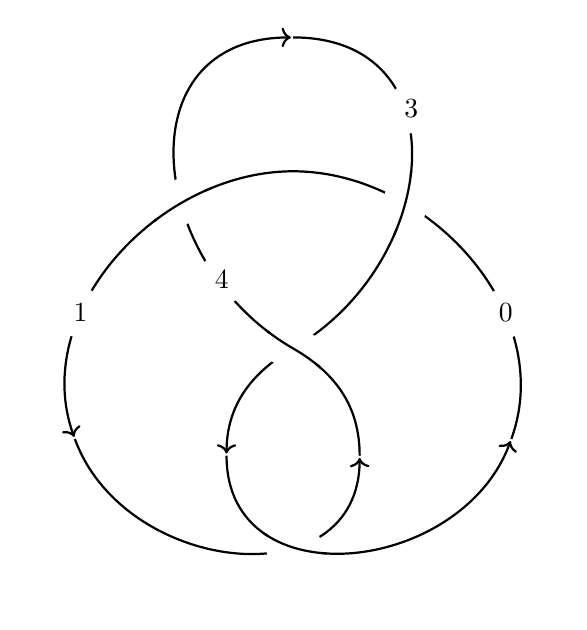
\begin{tikzpicture}[bgnd/.style={circle, fill=white, draw=white}]
      %\node[opacity=0.2] at (0,0) {\includegraphics[width=0.5\textwidth]{./rozdzialy/4_1-3d.png}};
      \coordinate (a1) at (90: 3.5);
      \coordinate (a2) at (-30:3.2);
      \coordinate (a3) at (210: 3.2);
      \coordinate (a4) at (0,-0.45);
      \coordinate (a5) at (-65:2);
      \coordinate (a6) at (180+65: 2);
      \coordinate (a7) at (90: 1.8);

      %\foreach \i in {1, ..., 7} \fill (a\i) circle (2pt);
      \begin{knot}[
        %consider self intersections,
        flip crossing=2,
        clip width=20,
        ]
        \strand[thick, ->]
        (a1) to [out=0, in=30, looseness=1.4]
        (a4) to [out=210, in=90, looseness=1] (a6);
        \strand[thick, ->]
        (a6) to [out=-90, in=250, looseness=1.3] (a2);
        \strand[thick, ->] (a2) to[out=70, in=0] (a7) to[out=180, in=110] (a3);
        \strand[thick, ->] (a3) to[out=290, in=-90, looseness=1.3] (a5);
        \strand[thick, ->] (a5) to[out=90, in=-30, looseness=1] (a4) to [out=150, in=180, looseness=1.4] (a1);
      \end{knot}

      \node[bgnd] at (60:3) {$3$};
      \node[bgnd] at (0:2.7) {$0$};
      \node[bgnd] at (-180:2.7) {$1$};
      \node[bgnd] at (155:1) {$4$};
    \end{tikzpicture}
    \caption{\label{fig:4_1:coloring} Coloring of knot $4_1$ with elements from $\Z_5$.}
  \end{figure}

  Now, consider a homomorphism $\Z[t, t^{-1}]\to \Z$ defined by $t\mapsto -1$. This yields a new matrix for $f$, with Smith's normal form:
  $$f=\begin{pmatrix}
    -1 & 0 & 0 & 0\\
    0 & 1 & 0 & 0\\
    0 & 0 & 5 & 0\\
    0 & 0 & 0 & 0
  \end{pmatrix}$$
  The matrix above hints at existence of a coloring with elements from $\Z_5$, one of which is presented in \cref{fig:4_1:coloring}.
\end{example}


\section{Reducing normal form of a matrix}

In \cref{coloring definition as kernel} we defined the coloring module of a diagram $D$ as the kernel of coloring homomorphism. We might also want to extend this homomorphism to a short exact sequence
\begin{center}
  \begin{tikzcd}
    0\arrow[r] & \ker f\arrow[r, hookrightarrow] & M^s\arrow[r, "f"] & M^s\arrow[r, two heads] & \coker f \arrow[r] & 0
  \end{tikzcd}
\end{center}
and ask what information can be obtained from studying $\coker f$.

In \cref{ex2,,ex3} nontrivial coloring was admissible only in modules $M/\mathfrak{a}$, where $\mathfrak{a}$ is the ideal spanned by a portion of terms that appear on the diagonal of Smith's normal form of $f$. In the same examples, we observe also that $\coker f=R^k\oplus R/\mathfrak{a}$. For the knot $3_1$ it was $\coker f=\Z\oplus \Z_3$, while in the case of knot $4_1$ $\coker f=\Z\oplus \Z_5$.

\begin{proposition}
  Let $f$ be a coloring homomorphism of an oriented diagram $D$. If $\coker f=R/\mathfrak{a}_1\oplus...\oplus R/\mathfrak{a}_k$ then $D$ can be colored with elements from $R/\mathfrak{a}_i$ for $i=1,..., k$.
\end{proposition}

\begin{proof}
  {\color{red}To się powinno sprowadzić do rozwiązywania układu równań przy pomocy macierzy}.
\end{proof}

The coloring homomorphism $f$ of a diagram $D$ carries a lot of information about the knot whose diagram it is. However, $f$ in itself is not a knot invariant. The dimensions of its matrix will change if a new crossing is created, see the following example.

\begin{example}\label{ex4}
  We take knot $3_1$ with additional crossing, $R=\Z[t, t^{-1}]$ and $M=\Z[t, t^{-1}]$ with $\phi$ as in \cref{ex3}. The coloring homomorphism has matrix
  $$
  \begin{pmatrix}
    1-t & t & -1 & 0 \\ 
    t & -1 & 0 & 1-t \\ 
    -1 & 1-t & 0 & t \\ 
    0 & 0 & 1 & -1 
  \end{pmatrix}
  $$
  with normal form
  $$
  \begin{pmatrix}
    -1 & 0 & 0 & 0\\ 
    0 & 1 & 0 & 0 \\ 
    0 & 0 & -t^2+t-1 & 0 \\ 
    0 & 0 & 0 & 0 &
  \end{pmatrix}
  $$
  which after evaluation at $t=-1$ yields
  $$
  \begin{pmatrix}
    -1 & 0 & 0 & 0\\ 
    0 & 1 & 0 & 0 \\ 
    0 & 0 & -3 & 0 \\ 
    0 & 0 & 0 & 0 &
  \end{pmatrix}
  $$
  which differs from matrix obtained in \cref{ex2} by just one trivial.
  \begin{figure}[h]\centering 
    \begin{tikzpicture}
    \begin{knot}[
      clip width=40,
      consider self intersections,
      ignore endpoint intersections=false, 
      flip crossing=2
      ]
      \strand[thick, ->] 
        (90:3) to [out=180, in=-90-30, looseness=2] 
        (-30:3);
      \strand[thick, ->] (-30:3) to [out=60, in=90, looseness=1.5] 
        (200:3.5); 
      \strand[thick, ->] (200:3.5) to[out=-90, in=-30, looseness=1.5] 
        (210:5);
      \strand[thick, ->] (210:5) to[out=180-30, in=180-30, looseness=1.5] 
        (210:3); 
      \strand[thick, ->] (210:3) to[out=-30, in=0, looseness=2]
        (90:3);
    \end{knot}
    \end{tikzpicture}
    \caption{Diagram of knot $3_1$ with additional crossing.\label{trefoil z dodatkowym skrzyzowaniem}}
  \end{figure}
\end{example}

The nontrivial term on the diagonal in \cref{ex4} is the same as in \cref{ex2}. The difference between matrices obtained in those two examples are their dimensions.

\begin{definition}\label{equivalence of matrices definition}
  % Let $f$ be a coloring homomorphism of diagram $D$ with Smith's normal form 
  % $$
  % S=\begin{pmatrix}
  %   a_1 & 0 & 0 & \hdots & 0 & \hdots & 0 \\ 
  %   0 & a_2 & 0\\ 
  %   0 & 0  & \ddots & & \vdots & & \vdots \\ 
  %       & & & a_k \\ 
  %     0 & &\hdots &  & 0 & \hdots & 0 \\ 
  %     \vdots & & & & \vdots & & \vdots\\ 
  %     0 & & \hdots & & 0 & \hdots & 0
  %   \end{pmatrix}
  % $$
  % We will define 
  %
  %
  Let $A$, $B$ be matrices with entries from a PID ring $R$. We will say that they are equivalent ($A\sim B$) if and only if their Smith's normal form has the same nonzero and nonunit terms.
\end{definition}

\begin{example}
  Matrices of coloring homomorphisms over the ring $\Z$ of knot $3_1$ presented in \cref{ex2,,ex4} are both equivalent to a $1\times 1$ matrix $\begin{pmatrix}3\end{pmatrix}$.
\end{example}

\begin{theorem}
  Equivalence class of matrices under relation $\sim$ defined in \cref{equivalence of matrices definition} is a knot invariant.
\end{theorem}







\bigskip

\rule{\textwidth}{1pt}
\bigskip

\begin{example} 
  First, consider the knot $6_1$ with diagram as seen in \cref{fig:6_1:knot}, ring $R=\Z[t, t^{-1}]$ and $M=R$. We calculate that
\begin{figure}[h]\centering
  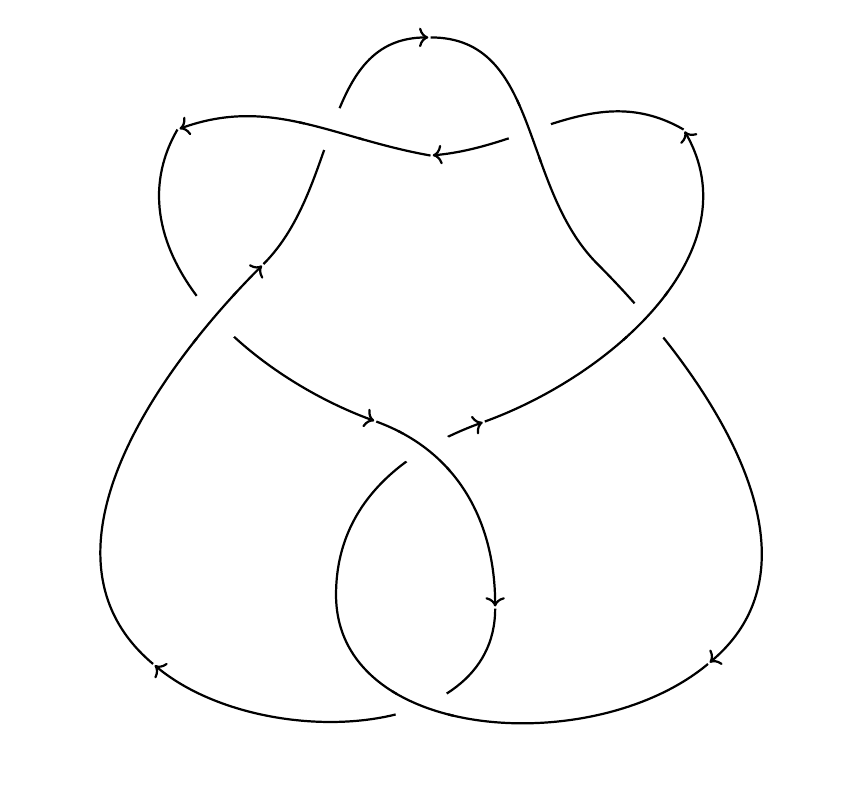
\begin{tikzpicture}[bgnd/.style={circle, fill=white, draw=white}]
    %\node[opacity=0.2] at (0,0) {\includegraphics[width=0.7\textwidth]{./rozdzialy/6_1-3d.png}};

    \coordinate (a0) at (0,0);
    \coordinate (a1) at (90:5);
    \coordinate (a2) at (45:3);
    \coordinate (a3) at (-40:4.6);
    \coordinate (a4) at (-120:2.4);
    \coordinate (a5) at (10:0.7);
    \coordinate (a6) at (50:5);
    \coordinate (a7) at (90:3.5);
    \coordinate (a8) at (180-50:5);
    \coordinate (a9) at (170:0.7);
    \coordinate (a10) at (-70:2.4);
    \coordinate (a11) at (220:4.6);
    \coordinate (a12) at (180-45:3);

    %\foreach \i in {0,...,12} \fill (a\i) circle (2pt);

    \begin{knot}[
      clip width=20, 
      flip crossing=1,
      flip crossing=3,
      flip crossing=6
      ]
      \strand[thick, ->] (a1) to[out=0, in=90+45] (a2) to[out=-45, in=40] (a3);
      \strand[thick, ->] (a3) to[out=220, in=-90] (a4) to[out=90, in=200] (a5);
      \strand[thick, ->] (a5) to[out=20, in=-60] (a6);
      \strand[thick, ->] (a6) to[out=150, in=5] (a7);
      \strand[thick, ->] (a7) to[out=170, in=20] (a8);
      \strand[thick, ->] (a8) to[out=240, in=160] (a9);
      \strand[thick, ->] (a9) to[out=-20, in=90] (a10);
      \strand[thick, ->] (a10) to[out=-90, in=-40] (a11);
      \strand[thick, ->] (a11) to[out=140, in=180+45] (a12);
      \strand[thick, ->] (a12) to[out=45, in=180] (a1);
    \end{knot}

    %\node at (80: 5) {$A$};
    %\node at (-40:4) {$B$};
    %\node at (45:5.5) {$C$};
    %\node at (135:5.5) {$D$};
    %\node at (-1.5,0.1) {$E$};
    %\node at (220:4) {$F$};
    %
    %\node[bgnd] at (70:4.7) {$1$};
    %\node[bgnd] at (25:3.9) {$2$};
    %\node[bgnd] at (-90:3) {$3$};
    %\node[bgnd] at (90:0.5) {$4$};
    %\node[bgnd] at (110:4.7) {$5$};
    %\node[bgnd] at (180-25:3.9) {$6$};

    %\draw[dashed] (70: 4) circle (0.4);
    %\draw[dashed] (28: 3.1) circle (0.4);
    %\draw[dashed] (-90:3.5) circle (0.4);
    %\draw[dashed] (-90:0.15) circle (0.4);
    %\draw[dashed] (180-28:3.1) circle (0.4);
    %\draw[dashed] (110:4) circle (0.4);
  \end{tikzpicture}
  \caption{\label{fig:6_1:knot}Diagram of knot $6_1$.}
\end{figure}
$$f=\begin{pmatrix}
  -1 & 0 & 0 & 0 & 0 & 0 \\ 
  0 & -1 & 0 & 0 & 0 & 0 \\ 
  0 & 0 & t & 0 & 0 & 0 \\ 
  0 & 0 & 0 & t & 0 & 0 \\ 
  0 & 0 & 0 & 0 & -2t^{-2}+5t^{-1}-2 & 0 \\ 
  0 & 0 & 0 & 0 & 0 & 0 
\end{pmatrix}$$
which agrees with the Alexander polynomial of $6_1$. Now, the reduced form of $f$ would be 
$$
\begin{pmatrix}
  -2t^{-2}+5t^{-1}-2
\end{pmatrix}
$$
a $1\times 1$ matrix.

There is another knot with Alexander polynomial equal $-2t^{-2}+5t^{-1}-2$: $9_{46}$. Using diagram in \cref{fig:9_46:knot} it can be calculated that  
\begin{figure}[h]\centering
  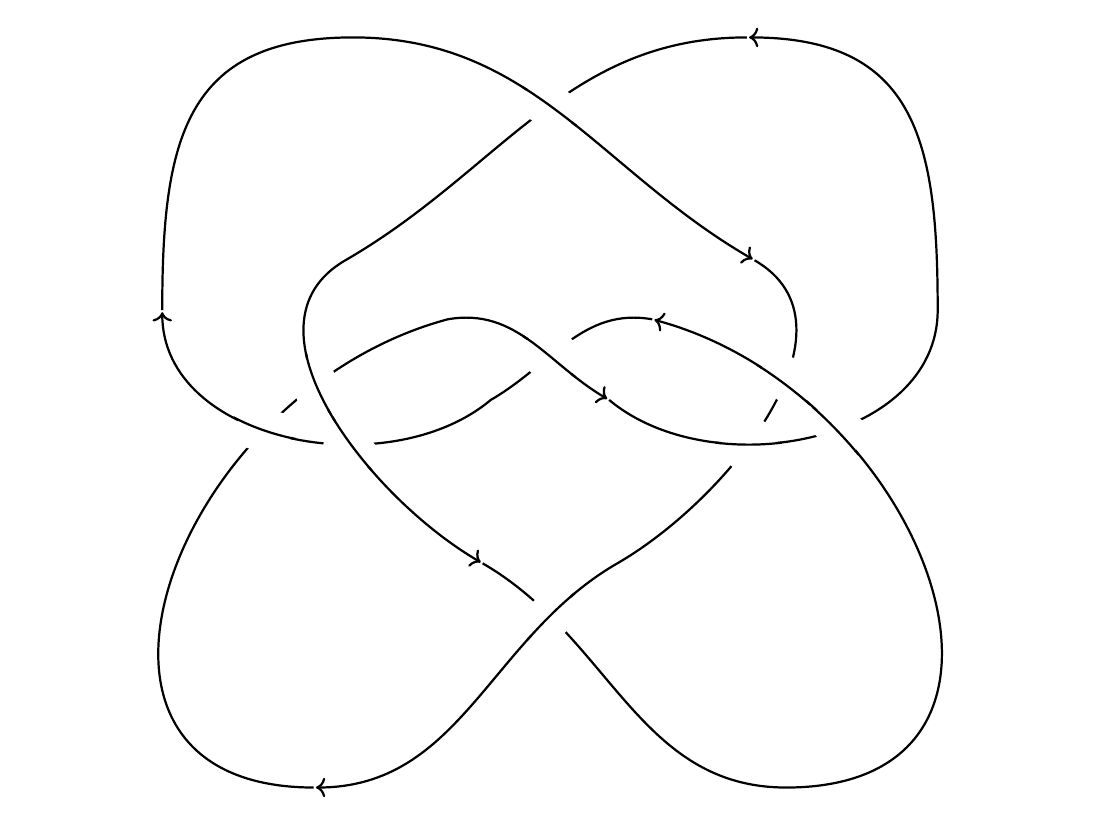
\begin{tikzpicture}[bgnd/.style={circle, fill=white, draw=white}]
    %\node[opacity=0.2] at (0,0) {\includegraphics[width=0.7\textwidth]{./rozdzialy/6_1-3d.png}};

    \coordinate (a0) at (0,0);
    \coordinate (a1) at (60:5);
    \coordinate (a2) at (150:3);
    \coordinate (a3) at (-110:2.5);
    \coordinate (a4) at (-60:6);
    \coordinate (a5) at (30:1.5);
    \coordinate (a6) at (200:0.8);
    \coordinate (a7) at (170:5);
    \coordinate (a8) at (120:5);
    \coordinate (a9) at (30:3);
    \coordinate (a10) at (-70:2.5);
    \coordinate (a11) at (180+60:6);
    \coordinate (a12) at (150:1.5);
    \coordinate (a13) at (-20:0.8);
    \coordinate (a14) at (10:5);

    %\foreach \i in {0,...,14} \fill (a\i) circle (2pt);

    \begin{knot}[
      clip width=20, 
      consider self intersections,
      ignore endpoint intersections=false,
      %draft mode=crossings,
      flip crossing=1,
      flip crossing=4,
      flip crossing=7, 
      flip crossing=9
      ]
      \strand[thick, ->] 
        (a1) to [out=180, in=30]
        (a2) to [out=210, in=150]
        (a3);
      \strand[thick, ->]
        (a3) to [out=-30, in=180] 
        (a4) to [out=0, in=-15, looseness=1.5] 
        (a5);
      \strand[thick, ->]
        (a5) to [out=170, in=30] 
        (a6) to [out=220, in=-90] 
        (a7);
      \strand[thick, ->]
        (a7) to [out=90, in=180, looseness=1.3] 
        (a8) to [out=0, in=150] 
        (a9);
      \strand[thick, ->]
        (a9) to [out=-30, in=30]
        (a10) to [out=210, in=0] 
        (a11);
      \strand[thick, ->]
        (a11) to [out=180, in=180+15, looseness=1.5] 
        (a12) to [out=10, in=150]
        (a13);
      \strand[thick, ->]
        (a13) to [out=-40, in=-90]
        (a14) to [out=90, in=0, looseness=1.3]
        (a1);
      \fill[yellow] (-10:3.7) circle (6pt);
    \end{knot}
  \end{tikzpicture}
  \caption{\label{fig:9_46:knot}Diagram of knot $9_{46}$.}
\end{figure}
$$f=\begin{pmatrix}
  1 & 0 & 0 & 0 & 0 & 0 & 0 & 0 & 0 \\ 
  0 & t^{-1} & 0 & 0 & 0 & 0 & 0 & 0 & 0 \\ 
  0 & 0 & t^{-1} & 0 & 0 & 0 & 0 & 0 & 0\\ 
  0 & 0 & 0 & t  & 0 & 0 & 0 & 0 & 0 \\ 
  0 & 0 & 0 & 0 & t  & 0 & 0 & 0 & 0 \\ 
  0 & 0 & 0 & 0 & 0 & t  & 0 & 0 & 0\\ 
  0 & 0 & 0 & 0 & 0 & 0 & 2t-t^2 & 0 & 0 \\ 
  0 & 0 & 0 & 0 & 0 & 0 & 0 & t^{-2}-2t^{-1} & 0\\ 
  0 & 0 & 0 & 0 & 0 & 0 & 0 & 0 & 0
\end{pmatrix}$$
where 
$$\det f= (2t-t^2)(t^{-2}-2t^{-1})=2t^{-1}-5+2t$$
is also the Alexander polynomial. The reduced form of $f$ is
$$
\begin{pmatrix}
  2t-t^2 & 0 \\ 
  0      & t^{-2}-2t^{-1}
\end{pmatrix}
$$
which is significantly different than the one for $6_1$.
\end{example}

{\large\color{red}TO DO: sprawdzić te węzły wyżej za pomocą pow. Seiferta, czy mają różne moduły Alexandera}


\bibliographystyle{plain}
\bibliography{literatura}
 
\end{document}
